\documentclass[a4paper,12pt]{scrreprt}
\usepackage{graphicx}       % Per le immagini


% === Pacchetti utili ===
\usepackage[utf8]{inputenc}       % Codifica dei caratteri
\usepackage[T1]{fontenc}          % Font encoding
\usepackage[italian]{babel}       % Lingua italiana
\usepackage{graphicx}             % Immagini
\usepackage{hyperref}             % Collegamenti ipertestuali
\usepackage{listings}             % Codice (in alternativa a minted)
\usepackage{xcolor}               % Colori per codice
\usepackage{lmodern}  % Versione moderna di Computer Modern Roman
\usepackage{needspace} % usata per avere più spazio all'occorrenza
\usepackage[normalem]{ulem} % sottolineatura colorata su testo colorato


% Uniforma lo stile dei titoli al testo principale (senza cambiare font)
\setkomafont{title}{\normalfont\bfseries\Huge}
\setkomafont{subtitle}{\normalfont\bfseries\Large}
\setkomafont{author}{\normalfont\bfseries\normalsize}
\setkomafont{chapter}{\normalfont\bfseries\Huge}
\renewcommand{\chapterformat}{\thechapter.\enskip}
\setkomafont{section}{\normalfont\bfseries\Large}
\renewcommand{\sectionformat}{\thesection\enspace\textendash\enskip}
\setkomafont{subsection}{\normalfont\bfseries\normalsize}


% === Stile per codice ===
\lstset{
  basicstyle=\ttfamily\small,
  backgroundcolor=\color{white},
  frame=single,
  breaklines=true,
  captionpos=b
}

% === definizione di colori custom === %
\definecolor{darkorange}{RGB}{205,105,0}
\definecolor{darkblue}{RGB} {0,0,200}

% Sottolineatura colorata
\newcommand{\ulred}[1]{\bgroup\markoverwith{\textcolor{red}{\rule[-0.5ex]{2pt}{0.4pt}}}\ULon{#1}\egroup}
\newcommand{\ulblue}[1]{\bgroup\markoverwith{\textcolor{blue}{\rule[-0.5ex]{2pt}{0.4pt}}}\ULon{#1}\egroup}
\newcommand{\ulorange}[1]{\bgroup\markoverwith{\textcolor{darkorange}{\rule[-0.5ex]{2pt}{0.4pt}}}\ULon{#1}\egroup}
\newcommand{\ulgreen}[1]{\bgroup\markoverwith{\textcolor{green!60!black}{\rule[-0.5ex]{2pt}{0.4pt}}}\ULon{#1}\egroup}

% Stile per SQL
\lstdefinelanguage{SQL}{
    morekeywords={CREATE,VIEW,AS,SELECT,FROM,WHERE,JOIN,ON,AND,OR,IN,IS,NULL,NOT,EXISTS,TABLE,AUTO_INCREMENT,PRIMARY,FOREIGN,CONSTRAINT,KEY,DELETE,CASCADE,UPDATE,REFERENCES,DEFAULT,UNIQUE},
    sensitive=false,
    morecomment=[l]{--},
    morestring=[b]',
}

\lstset{
    language=SQL,
    basicstyle=\ttfamily\small,
    keywordstyle=\color{darkblue}\bfseries,
    commentstyle=\color{gray}\itshape,
    stringstyle=\color{darkorange},
    columns=flexible,
    breaklines=true,
    showstringspaces=false,
    frame=none
}


\title{Documentazione TIW}
\subtitle{Traccia 3 24-25}
\author{Cristianelli Ennio - De Giorgio Domenico}
\date{}

\begin{document}

\maketitle

\tableofcontents

\chapter{Analisi delle specifiche}
\section{Specifiche generali}
\begin{center}
  \textcolor{red}{\textbf{Entità}},
  \textcolor{green!60!black}{\textbf{Attributi}},
  \textcolor{blue}{\textbf{Relazioni}}
\end{center}
\noindent Un’applicazione permette di verbalizzare gli esiti degli esami di un appello. Il \textcolor{red}{docente} accede tramite login e
\textcolor{blue}{seleziona} nella HOME page \textcolor{blue}{un corso da una lista dei propri corsi}, ordinata per nome del corso in modo alfabetico
decrescente, e poi sceglie una \textcolor{green!60!black}{data} d’\textcolor{red}{appello} \textcolor{blue}{del corso} scelto da un elenco ordinato per data decrescente. Ogni
\textcolor{red}{corso} \textcolor{blue}{ha un solo docente}. La selezione dell’appello porta a una pagina ISCRITTI, che mostra una tabella con tutti gli
iscritti all’appello. La tabella riporta i seguenti dati: \textcolor{green!60!black}{matricola, cognome e nome, email, corso di laurea, voto e stato
di valutazione}. Il voto può non essere ancora definito. Lo stato di valutazione dello studente rispetto all’appello può
assumere i valori: non inserito, inserito, pubblicato, rifiutato e verbalizzato. Selezionando un’etichetta
nell’intestazione della tabella, l’utente ordina le righe in base al valore di tale etichetta (ad esempio, selezionando
“cognome” la tabella è riordinata in base al cognome). Successive selezioni della stessa etichetta invertono
l’ordinamento: si parte con l’ordinamento crescente. Il valore del voto viene considerato ordinato nel modo
seguente: <vuoto>, assente, rimandato, riprovato, 18, 19, …, 30, 30 e lode. Nella tabella della pagina ISCRITTI ad
ogni riga corrisponde un bottone “MODIFICA”. Premendo il bottone compare una pagina con una form che mostra
tutti i dati dello studente selezionato e un campo di input in cui è possibile scegliere il voto. L’invio della form
provoca la modifica o l’inserimento del voto. Inizialmente le righe sono nello stato di valutazione “non inserito”.
L’inserimento e le successive eventuali modifiche portano la riga nello stato di valutazione “inserito”. Alla tabella
della pagina ISCRITTI è associato un bottone PUBBLICA che comporta la pubblicazione delle righe con lo stato di
valutazione INSERITO. La pubblicazione rende il voto non più modificabile dal docente e visibile allo studente e
cambia lo stato di valutazione della riga dello studente a “pubblicato”. Lo \textcolor{red}{studente} accede tramite login e \textcolor{blue}{seleziona}
nella HOME page \textcolor{blue}{un corso tra quelli a cui è iscritto} mediante una lista ordinata in modo alfabetico decrescente e
poi una data d’appello del corso scelto selezionata da un elenco ordinato per data decrescente. \textcolor{blue}{Uno studente può
essere iscritto a più appelli dello stesso corso}. La selezione della data d’appello porta a una pagina ESITO che mostra
il messaggio “Voto non ancora definito” se il docente non ha ancora pubblicato il risultato per quello studente in
quell’appello. Altrimenti, la pagina mostra i dati dello studente, del corso, dell’appello e il voto assegnato. Se il voto
è tra 18 e 30 e lode compare un bottone RIFIUTA. Premendo tale bottone la pagina mostra gli stessi dati con la
dizione aggiunta “Il voto è stato rifiutato” e senza il bottone RIFIUTA. Il rifiuto del voto cambia lo stato di valutazione
a “rifiutato” della riga dello studente per quell’appello nella pagina ISCRITTI del docente. Nella pagina ISCRITTI del
docente la tabella degli iscritti è associata anche a un bottone VERBALIZZA. La pressione del bottone provoca il
cambio di stato a “verbalizzato” per le righe nello stato “pubblicato” o "rifiutato" e comporta anche la \textcolor{blue}{creazione} di
un \textcolor{red}{verbale} e la disabilitazione della possibilità di rifiutare il voto. Il rifiuto implica la verbalizzazione di “rimandato”
come voto. Un verbale ha \textcolor{green!60!black}{un codice generato dal sistema, una data e ora di creazione} ed \textcolor{blue}{è associato all’appello del
corso a cui si riferisce e agli studenti} (con nome, cognome, matricola e voto) che passano allo stato “verbalizzato”.
A seguito della pressione del bottone VERBALIZZA compare una pagina VERBALE che mostra i dati completi del
verbale creato. Il docente dispone anche di una pagina VERBALI, in cui sono elencati tutti i verbali da lui creati,
ordinati on modo alfabetico crescente per nome del corso e poi per data crescente di appello di ogni corso.

\section{Versione javascrypt}
Si realizzi un’applicazione client server web che modifica le specifiche precedenti come segue:
\begin{itemize}
    \item Dopo il login dell’utente, l’intera applicazione è realizzata con un’unica pagina per il docente e un’unica pagina per lo studente.
    \item Ogni interazione dell’utente è gestita senza ricaricare completamente la pagina, ma produce l’invocazione
    asincrona del server e l’eventuale modifica del contenuto da aggiornare a seguito dell’evento.
    \item La funzione di riordino della tabella degli iscritti è realizzata a lato client.
    \item La funzione di rifiuto del voto da parte dello studente è realizzata mediante trascinamento del testo
    corrispondente all’esito (dati dello studente, del corso, dell’appello e voto assegnato) sopra un’icona che
    rappresenta il cestino. Al rilascio compare una messaggio popup che chiede di confermare l’operazione di
    rifiuto, con due bottoni (CANCELLA, CONFERMA). Il primo ripristina la situazione precedente al trascinamento,
    il secondo effettua l’operazione di rifiuto.
    \item Alla tabella degli iscritti è associato un bottone INSERIMENTO MULTIPLO che provoca la comparsa di una
    pagina modale con tutte e sole le righe nello stato “non inserito” associate a un campo di input. Il docente può
    inserire un voto per un insieme delle righe e premere un bottone INVIA che comporta l’invio al server dei voti,
    il cambio di stato delle righe coinvolte, la chiusura della finestra modale e l’aggiornamento della tabella degli
    iscritti.
\end{itemize}

\newpage
\chapter{Progettazione del database}
\section{Diagramma Entità Relazione}
\begin{figure}[htbp]
    \centering
    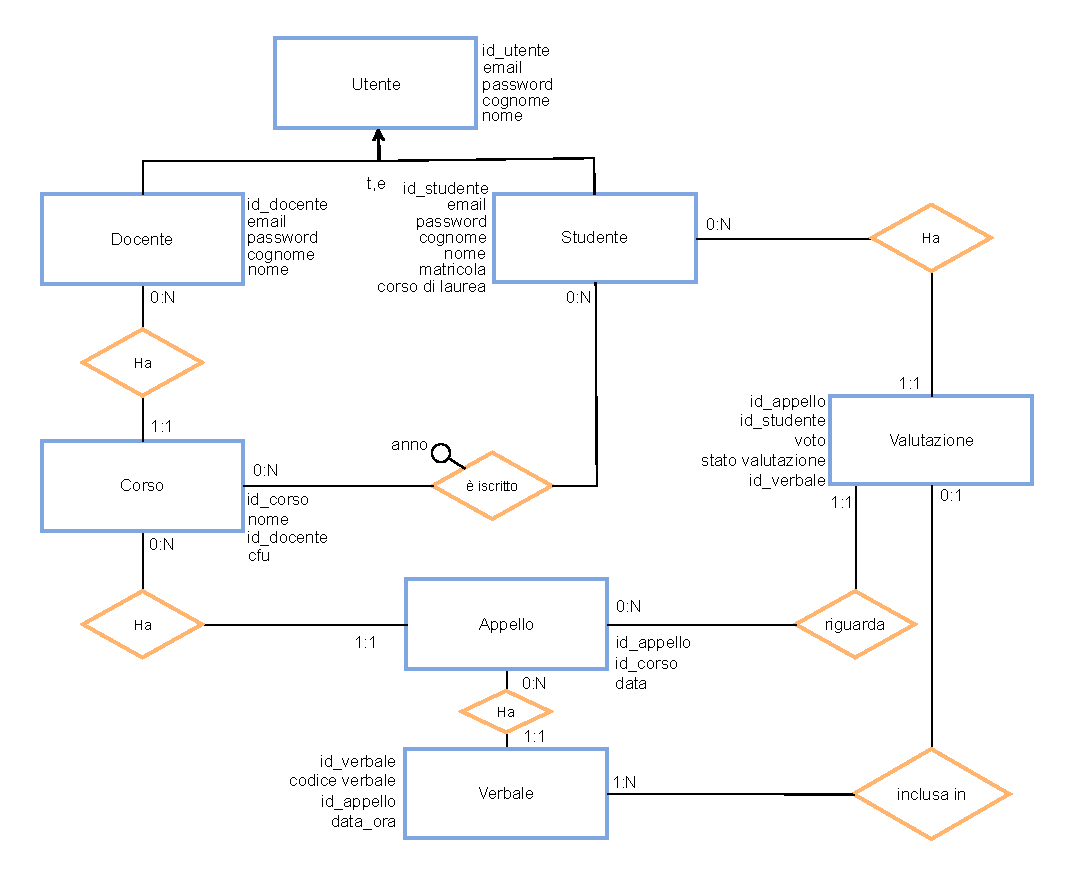
\includegraphics[width=1.0\textwidth]{diagrammaER.drawio.pdf}
\end{figure}

\newpage

\section{Schema del database}


\begin{lstlisting}
    CREATE TABLE 'utente' (
    'id_utente' int NOT NULL AUTO_INCREMENT,
    'email' varchar(100) NOT NULL,
    'password' varchar(50) NOT NULL,
    'cognome' varchar(30) NOT NULL,
    'nome' varchar(30) NOT NULL,
    PRIMARY KEY ('id_utente')
    )
\end{lstlisting}

\begin{lstlisting}
    CREATE TABLE 'docente' (
    'id_docente' int NOT NULL,
    PRIMARY KEY ('id_docente'),
    CONSTRAINT 'fk_docente_utente' FOREIGN KEY ('id_docente') REFERENCES 'utente' ('id_utente') ON DELETE CASCADE ON UPDATE CASCADE
    )
\end{lstlisting}


\begin{lstlisting}
    CREATE TABLE 'studente' (
    'id_studente' int NOT NULL,
    'matricola' varchar(45) NOT NULL,
    'corso_laurea' varchar(45) NOT NULL, 
    PRIMARY KEY ('id_studente'),
    UNIQUE KEY 'matricola_UNIQUE' ('matricola'),
    CONSTRAINT 'fk_studente_utente' FOREIGN KEY ('id_studente') REFERENCES 'utente' ('id_utente') ON DELETE CASCADE ON UPDATE CASCADE
    )
\end{lstlisting}

\begin{lstlisting}
    CREATE TABLE 'corso' (
    'id_corso' int NOT NULL AUTO_INCREMENT,
    'nome' varchar(45) NOT NULL,
    'cfu' int NOT NULL,
    'id_docente' int NOT NULL,
    PRIMARY KEY ('id_corso'),
    KEY 'idx_docente' ('id_docente'),
    CONSTRAINT 'fk_corso_docente' FOREIGN KEY ('id_docente') REFERENCES 'docente' ('id_docente') ON DELETE CASCADE ON UPDATE CASCADE
    )
\end{lstlisting}

\Needspace{11\baselineskip}

\begin{lstlisting}
    CREATE TABLE 'iscrizione_corso' (
    'id_studente' INT NOT NULL,
    'id_corso' int NOT NULL,
    'anno' year NOT NULL,
    PRIMARY KEY ('id_studente','id_corso','anno'),
    KEY 'iscr_corso' ('id_corso'),
    CONSTRAINT 'fk_iscr_corso' FOREIGN KEY ('id_corso') REFERENCES corso ('id_corso') ON DELETE CASCADE ON UPDATE CASCADE,
    CONSTRAINT 'fk_iscr_studente' FOREIGN KEY ('id_studente') REFERENCES studente ('id_studente') ON DELETE CASCADE ON UPDATE CASCADE
    )
\end{lstlisting}


\begin{lstlisting}
    CREATE TABLE 'appello' (
    'id_appello' int NOT NULL AUTO_INCREMENT,
    'id_corso' int NOT NULL,
    'data' date NOT NULL,
    PRIMARY KEY ('id_appello'),
    KEY 'idx_corso' ('id_corso'),
    CONSTRAINT 'fk_appello_corso' FOREIGN KEY ('id_corso') REFERENCES 'corso' ('id_corso') ON DELETE CASCADE ON UPDATE CASCADE
    )
\end{lstlisting}

\begin{lstlisting}
    CREATE TABLE 'valutazione' (
    'id_studente' int NOT NULL,
    'id_appello' int NOT NULL,
    'voto' enum('','assente','rimandato','riprovato','18','19','20','21','22','23','24','25','26','27','28','29','30','30L') NOT NULL DEFAULT '',
    'stato_valutazione' enum('non inserito','inserito','pubblicato','rifiutato','verbalizzato') NOT NULL DEFAULT 'non inserito', 
    'id_verbale' int,
    PRIMARY KEY ('id_studente','id_appello'),
    KEY 'idx_appello' ('id_appello'),
    KEY 'idx_studente' ('id_studente'),
    CONSTRAINT fk_val_studente FOREIGN KEY ('id_studente') REFERENCES studente('id_studente') ON DELETE CASCADE ON UPDATE CASCADE,
    CONSTRAINT fk_val_appello FOREIGN KEY ('id_appello') REFERENCES appello('id_appello') ON DELETE CASCADE ON UPDATE CASCADE,
    CONSTRAINT fk_val_verbale FOREIGN KEY ('id_verbale') REFERENCES verbale('id_verbale') ON DELETE CASCADE ON UPDATE CASCADE
    )
\end{lstlisting}

\Needspace{11\baselineskip}


\begin{lstlisting}
    CREATE TABLE 'verbale' (
    'id_verbale' int NOT NULL AUTO_INCREMENT,
    'codice_verbale' int NOT NULL,
    'id_appello' int NOT NULL,
    'data_ora' datetime NOT NULL DEFAULT CURRENT_TIMESTAMP,
    PRIMARY KEY ('id_verbale'),
    KEY 'idx_appello' ('id_appello'),
    UNIQUE KEY 'verbale_UNIQUE' ('codice_verbale'),
    CONSTRAINT fk_verb_appello FOREIGN KEY ('id_appello') REFERENCES appello ('id_appello') ON DELETE CASCADE ON UPDATE CASCADE
    )
\end{lstlisting}

\newpage

\chapter{Progettazione dell'applicazione}
\section{Analisi dei requisiti}
\begin{center}
  \textcolor{red}{\textbf{Pages (views)}},
  \textcolor{green!60!black}{\textbf{view components}},
  \textcolor{blue}{\textbf{events,}}
  \textcolor{darkorange}{\textbf{actions}}
\end{center}
Un’applicazione permette di verbalizzare gli esiti degli esami di un appello. Il docente \textcolor{blue}{accede tramite} \textcolor{red}{\ulblue{login}} e
\textcolor{blue}{seleziona} nella \textcolor{red}{HOME page} \textcolor{blue}{un corso} da \textcolor{green!60!black}{una lista dei propri corsi, ordinata per nome del corso in modo alfabetico
decrescente}, e poi \textcolor{blue}{sceglie} \textcolor{green!60!black}{una data d’appello del corso} \textcolor{blue}{scelto} \textcolor{green!60!black}{da un elenco ordinato per data decrescente}. Ogni
corso ha un solo docente. \textcolor{blue}{La selezione dell’appello} porta a una \textcolor{red}{pagina ISCRITTI}, che \textcolor{green!60!black}{mostra una tabella con tutti gli
iscritti all’appello}. La tabella riporta i seguenti dati: matricola, cognome e nome, email, corso di laurea, voto e stato
di valutazione. Il voto può non essere ancora definito. Lo stato di valutazione dello studente rispetto all’appello può
assumere i valori: non inserito, inserito, pubblicato, rifiutato e verbalizzato. \textcolor{blue}{Selezionando} \textcolor{green!60!black}{un’etichetta
nell’intestazione della tabella}, \textcolor{darkorange}{l’utente ordina le righe in base al valore di tale etichetta} (ad esempio, selezionando
“cognome” la tabella è riordinata in base al cognome). \textcolor{blue}{Successive selezioni della stessa etichetta} \textcolor{darkorange}{invertono
l’ordinamento}: si parte con l’ordinamento crescente. Il valore del voto viene considerato ordinato nel modo
seguente: <vuoto>, assente, rimandato, riprovato, 18, 19, …, 30, 30 e lode. Nella tabella della pagina ISCRITTI \textcolor{green!60!black}{ad
ogni riga corrisponde un bottone} ''\textcolor{red}{\ulgreen{MODIFICA}}''. \textcolor{blue}{Premendo il bottone} compare una \textcolor{red}{pagina} con \textcolor{green!60!black}{un form che mostra
tutti i dati dello studente selezionato} e \textcolor{green!60!black}{una campo di input in cui è possibile scegliere il voto}.\textcolor{blue}{ L’invio della form}
\textcolor{darkorange}{provoca la modifica o l’inserimento del voto}. Inizialmente le righe sono nello stato di valutazione “non inserito”.
\textcolor{blue}{L’inserimento} e \textcolor{blue}{le successive eventuali modifiche} \textcolor{darkorange}{portano la riga nello stato di valutazione “inserito”}. Alla tabella
della pagina ISCRITTI è associato \textcolor{green!60!black}{un bottone PUBBLICA} che \textcolor{darkorange}{comporta la pubblicazione delle righe con lo stato di
valutazione INSERITO}. La pubblicazione rende il voto non più modificabile dal docente e visibile allo studente e
cambia lo stato di valutazione della riga dello studente a “pubblicato”. Lo studente \textcolor{blue}{accede tramite login} e \textcolor{blue}{seleziona}
nella \textcolor{red}{HOME page} \textcolor{green!60!black}{un corso tra quelli a cui è iscritto mediante una lista ordinata} in modo alfabetico decrescente e
\textcolor{green!60!black}{poi una data d’appello del corso scelto selezionata da un elenco ordinato} per data decrescente. Uno studente può
essere iscritto a più appelli dello stesso corso. \textcolor{blue}{La selezione della data d’appello} porta a una \textcolor{red}{pagina ESITO} che \textcolor{green!60!black}{mostra
il messaggio “Voto non ancora definito”} se il docente non ha ancora pubblicato il risultato per quello studente in
quell’appello. Altrimenti, la pagina \textcolor{green!60!black}{mostra i dati dello studente, del corso, dell’appello e il voto assegnato}. Se il voto
è tra 18 e 30 e lode compare \textcolor{green!60!black}{un bottone RIFIUTA}. \textcolor{blue}{Premendo tale bottone} la pagina \textcolor{darkorange}{mostra gli stessi dati con la
dizione aggiunta “Il voto è stato rifiutato” e senza il bottone RIFIUTA}. \textcolor{blue}{Il rifiuto del voto} \textcolor{darkorange}{cambia lo stato di valutazione
a “rifiutato”} della riga dello studente per quell’appello nella pagina ISCRITTI del docente. Nella pagina ISCRITTI del
docente la tabella degli iscritti è associata anche a \textcolor{green!60!black}{un bottone VERBALIZZA}. \textcolor{blue}{La pressione del bottone} \textcolor{darkorange}{provoca il
cambio di stato a “verbalizzato”} per le righe nello stato “pubblicato” o "rifiutato" e comporta anche la \textcolor{darkorange}{creazione di
un verbale} e \textcolor{darkorange}{la disabilitazione} della possibilità di rifiutare il voto. \textcolor{blue}{Il rifiuto} implica \textcolor{darkorange}{la verbalizzazione di “rimandato”
come voto}. Un verbale ha un codice generato dal sistema, una data e ora di creazione ed è associato all’appello del
corso a cui si riferisce e agli studenti (con nome, cognome, matricola e voto) che passano allo stato “verbalizzato”.
A seguito della \textcolor{blue}{pressione del bottone VERBALIZZA} compare una \textcolor{red}{pagina VERBALE} che \textcolor{green!60!black}{mostra i dati completi del}
\textcolor{darkorange}{\ulgreen{verbale creato}}. Il docente dispone anche di una \textcolor{red}{pagina VERBALI}, in cui \textcolor{green!60!black}{sono elencati tutti i verbali da lui creati},
ordinati on modo alfabetico crescente per nome del corso e poi per data crescente di appello di ogni corso.

\vspace{3em}

\section{Completamento delle specifiche}
\begin{itemize}
     \item La pagina di default è quella che contiene il form di login.
    \item Il login viene fatto tramite email e password e il sistema deve essere in grado di riconoscere tramite queste se l'utente è uno studente o un docente e mostrargli di conseguenza la propria HOME page.
    \item È possibile fare logout in qualunque momento, tornando alla schermata di login.
    \item È presente un bottone per tornare alla pagina precedente (comportamento di \textit{“indietro”}).
    \item Non si possono pubblicare voti se nessuna delle voci ha stato di valutazione ``inserito''.
    \item Non si possono verbalizzare voti se nessuna delle voci ha stato di valutazione ``pubblicato'' o ``rifiutato''.
    \item Una riga con stato ``pubblicato'' non può più essere modificata dal docente.
    \item Una riga con stato ``verbalizzato'' è da considerarsi definitiva e non modificabile.
    \item Il voto può essere modificato solo se lo stato è ``inserito'' o ``non inserito''.
    \item Il rifiuto di un voto da parte dello studente è possibile solo se il voto è tra 18 e 30 e lode, e se lo stato è ``pubblicato''.
    \item La verbalizzazione è un’operazione irreversibile.
    \item Il sistema mantiene una tracciatura delle operazioni eseguite (modifiche, pubblicazioni, rifiuti, verbalizzazioni).
    \item La selezione delle intestazioni di colonna permette di ordinare i dati; successive selezioni invertono l’ordine.
    \item L’ordinamento dei corsi e degli appelli è stabile e coerente con i criteri descritti (alfabetico decrescente per nome corso, cronologico decrescente per data d’appello).
    \item Dopo la verbalizzazione, il voto è visibile allo studente ma non più rifiutabile.
    \item Il bottone VERBALIZZA crea un verbale contenente solo le righe con stato ``pubblicato'' o ``rifiutato''.
    \item Il voto rifiutato da uno studente viene verbalizzato come ``rimandato''.
    \item Ogni verbale è identificato da un codice univoco generato automaticamente, una data e ora di creazione, ed è associato all’appello e agli studenti verbalizzati.
\end{itemize}

\section{Design dell'applicazione}

\subsection{Diagramma docente}
\begin{figure}[htbp]
    \centering
    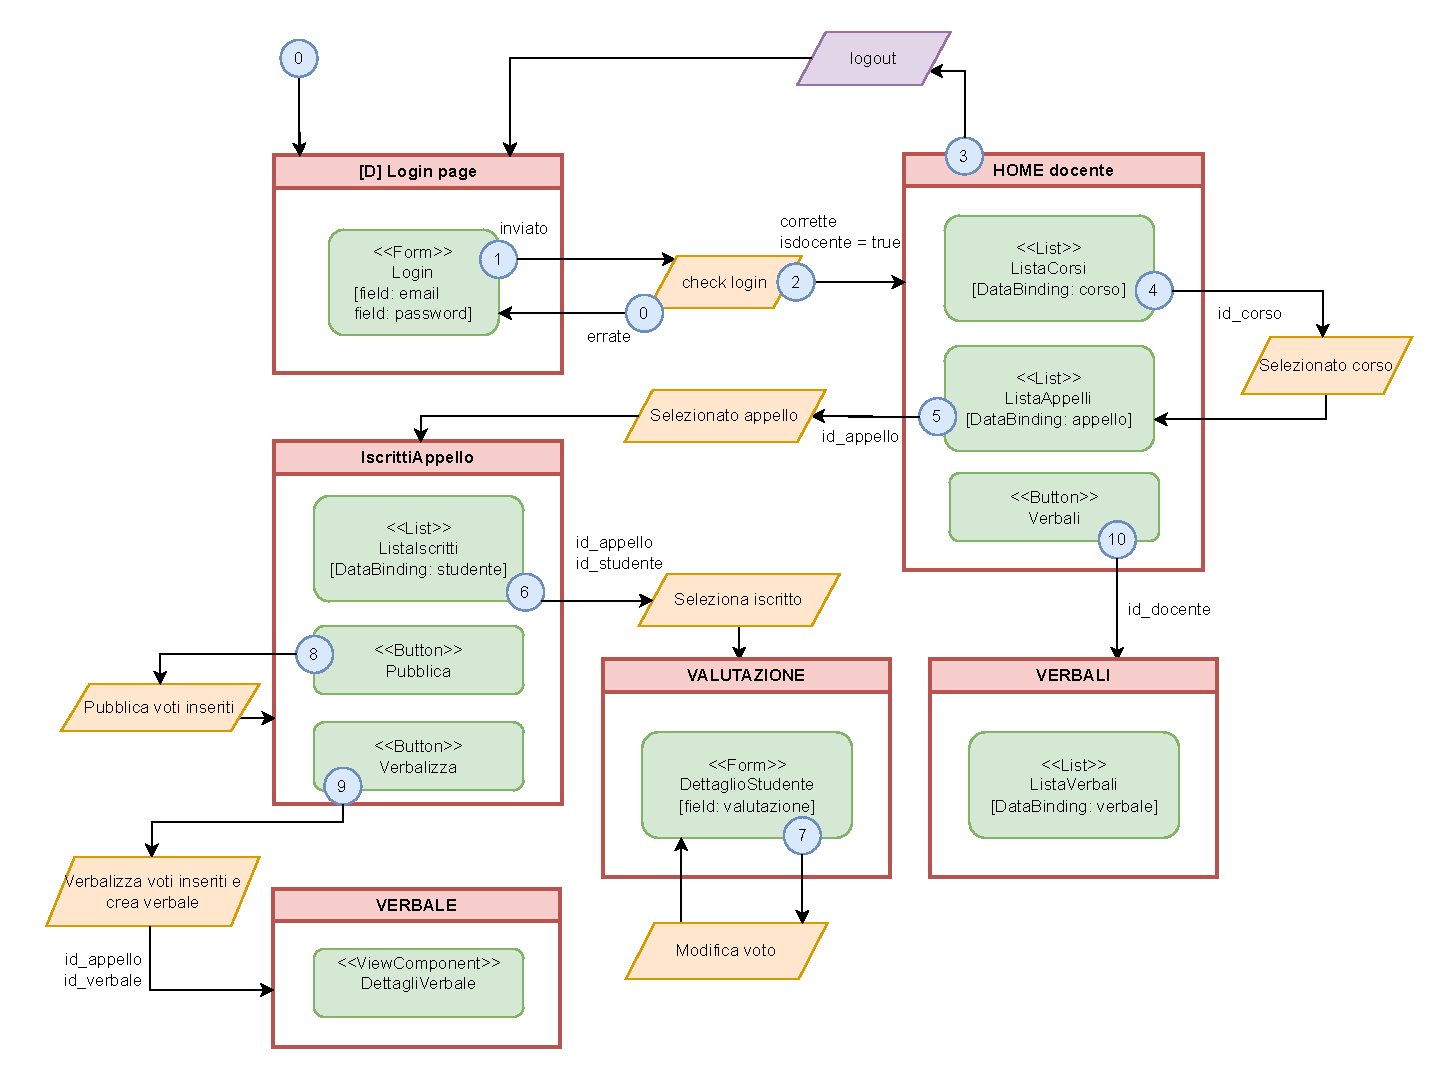
\includegraphics[width=0.8\textwidth]{docenteIFML.drawio.pdf}
    \caption{Diagramma IFML per il Docente}
\end{figure}

\newpage

\subsection{Diagramma studente}
\begin{figure}[htbp]
    \centering
    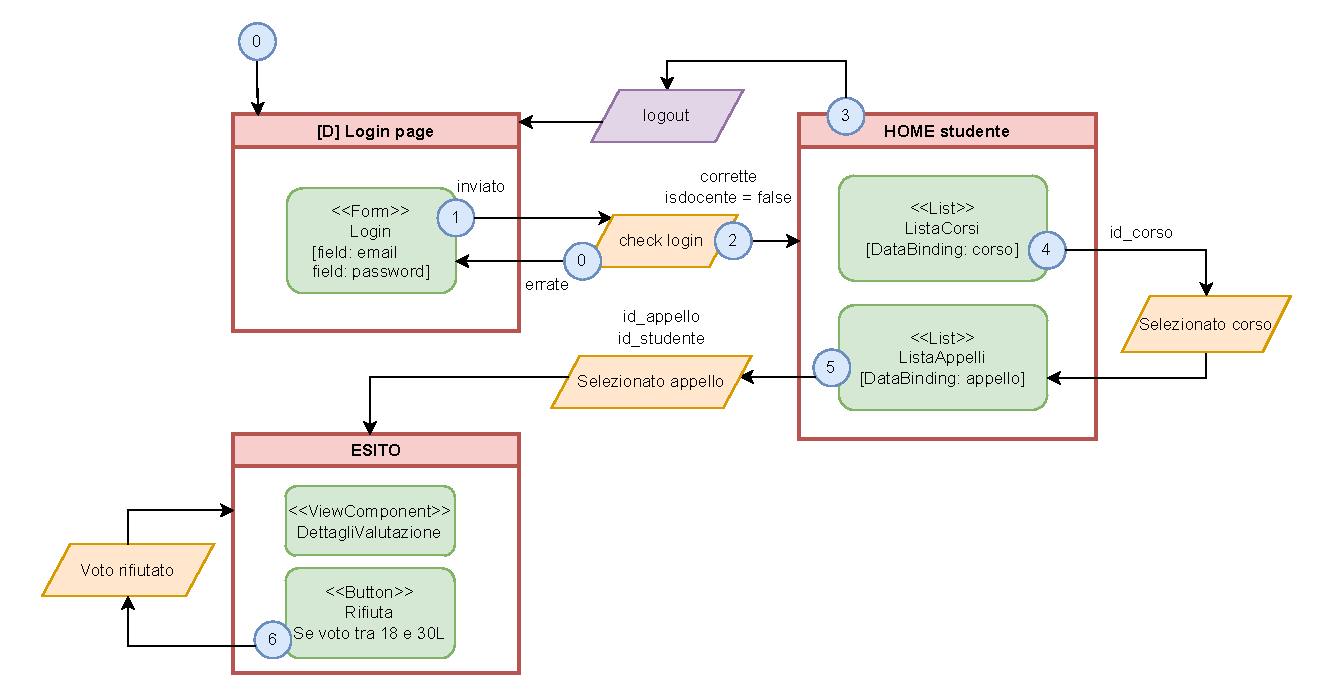
\includegraphics[width=0.8\textwidth]{studenteIFML.drawio.pdf}
    \caption{Diagramma IFML per lo Studente}
\end{figure}

\newpage

\section{Componenti}
\noindent
\begin{minipage}[t]{0.48\textwidth}
% --- Inizio colonna sinistra ---
\textbf{Model objects (beans)}
\begin{itemize}
    \item UtenteBean
    \item StudenteBean
    \item DocenteBean
    \item CorsoBean
    \item AppelloBean
    \item IscrizioneBean
    \item VerbaleBean
\end{itemize}
\textbf{Controllers (servlets)}
\begin{itemize}
    \item Frontend
    \begin{itemize}
        \item LoginServlet
        \item HomeServlet
        \item ModificaVotoServlet
        \item EsitoStudenteServlet
        \item VerbaliServlet
        \item VerbaleDettaglioServlet
        \item IscrittiAppelloServlet
    \end{itemize}
    \item Backend
    \begin{itemize}
        \item AutenticazioneServlet
        \item LogoutServlet
        \item SalvaVotoServlet
        \item VerbalizzaServlet
        \item PubblicaServlet
        \item RifiutaVotoServlet
    \end{itemize}
\end{itemize}

% --- Fine colonna sinistra ---
\end{minipage}
\hfill
\begin{minipage}[t]{0.48\textwidth}
% --- Inizio colonna destra ---
\textbf{Views (templates)}
\begin{itemize}
    \item login
    \item homeStudente
    \item homeDocente
    \item iscrittiAppello
    \item valutazione
    \item verbale
    \item verbali
    \item esito
\end{itemize}
\textbf{Data Access Objects (classes)}
\begin{itemize}
    \item UtenteDAO
    \begin{itemize}
            \item check credenziali 
    \end{itemize}
    \item DocenteDAO
    \begin{itemize}
            \item corsi
            \item appelli
            \item verbali
    \end{itemize}
    \item StudenteDAO
    \begin{itemize}
            \item corsi
            \item valutazioni
        \end{itemize}
    \item IscrizioneDAO
    \begin{itemize}
            \item stato valutazioni
            \item generazione verbale
            \item voti
            \item iscrizioni a un appello
    \end{itemize}
\end{itemize}
% --- Fine colonna destra ---
\end{minipage}


\end{document}
